\documentclass[11pt, a4paper]{article} %tamaño mínimo de letra 11pto.

% \usepackage{graphicx} 
\usepackage[spanish]{babel} %Español 
\usepackage[utf8]{inputenc} %Para poder poner tildes

\usepackage{vmargin} %Para modificar los márgenes
\setmargins{2.5cm}{1.5cm}{16.5cm}{23.42cm}{10pt}{1cm}{0pt}{2cm}
%margen izquierdo, superior, anchura del texto, altura del texto, altura de los encabezados, espacio entre el texto y los encabezados, altura del pie de página, espacio entre el texto y el pie de página

\usepackage[T1]{fontenc}


\renewcommand\familydefault{\rmdefault}  %% fuente 
\usepackage[a4paper, left=2.5cm, right= 2.5cm, top=2.5cm, bottom= 2.5cm]{geometry} %cambiar los márgenes
\usepackage{ amssymb, cancel, extarrows, amsmath, amsthm }%símbolos matemáticos
\usepackage{wasysym}  %la carita triste
\usepackage{derivative}
\usepackage{physics}

\newcommand{\D}[2][1]{\odif[order={#1}]{#2}} %% Notación de diferenciales con paquete derivative
\newcommand{\B}[1]{\mathbf{#1}}  %% Para hacer negrita sin escribir mathbf
\newcommand{\K}[2][]{\mathbb{#2}^{#1}} %%Letras chulas de espacios vectoriales y cuerpos
\newcommand{\Cl}[1]{\mathcal{#1}}  %%Letras caligráficas
\newcommand{\cte}{\text{const.}}

\usepackage{graphicx, wrapfig}% Include figure files
\usepackage{subfig}
\usepackage{dcolumn}% Align table columns on decimal point
\usepackage{bm}% bold math
\usepackage{hyperref}% add hypertext capabilities
\usepackage[spanish, es-tabla]{babel} %traducción al español
\addto{\captionspanish}{%
  \renewcommand*{\chaptername}{CAPÍTULO}
  \renewcommand*{\pagename}{PÁGINA}}
\usepackage{units}
\usepackage{fancyhdr, ragged2e}
\usepackage{anyfontsize}
\setlength{\headheight}{13.07002pt}
\renewcommand{\footrulewidth}{0.4pt}
\usepackage{float}
\usepackage{booktabs}
\usepackage[11pt]{moresize}
\usepackage{lipsum}
\usepackage{changepage}
\usepackage{calc}

\usepackage{multirow}
\usepackage{multicol}
\usepackage[table,xcdraw]{xcolor}
\usepackage{xcolor, colortbl}
\usepackage{pdfpages} %%insertar pdf dentro del documento
\usepackage{pagecolor}
\usepackage{tcolorbox}
\newtcolorbox{mybox}{colback=gray!5!white,colframe=black!75!black}
\definecolor{cadetblue4}{rgb}{.33,.53,.55}
\definecolor{azulcrepuscular}{rgb}{.49,.62,.75}
\definecolor {atomictangerine} {rgb} {1.0, 0.6, 0.4}
\definecolor{portada}{RGB}{2, 2, 0}
\usepackage{longtable}
\usepackage{hyperref}
\hypersetup{
    colorlinks=true,
    linkcolor=black,
    filecolor=magenta,      
    urlcolor=blue,
    pdftitle={Mec. Teo: Entregable 3},
    pdfpagemode=FullScreen,
    }

\usepackage{titlesec}
\titleformat{\chapter}[display]
  {\normalfont\rmfamily\huge\bfseries}
  {\chaptertitlename\ \thechapter}{20pt}{\Huge}[{\titlerule[2pt]}]
\titleformat*{\section}{\Large\normalfont\rmfamily\bfseries}
\titleformat*{\subsection}{\large\normalfont\rmfamily\bfseries}
\titleformat*{\subsubsection}{\normalsize\normalfont\rmfamily\bfseries} 

\usepackage{notomath}   %% fuente para entornos matemáticos

\setlength{\parindent}{0cm}  %% para quitar la sangría francesa esa repulsiva

\newcounter{define}[section] %%contador para definiciones

\newenvironment{define}[1][]{\refstepcounter{define}\underline{\textbf{Definición \thedefine}} [#1]: \ \begin{minipage}[t]{\textwidth-\widthof{\underline{\textbf{Definición \thedefine}}["\emph{#1}"]:}}}{\end{minipage}\\\\}  %%definicion de entorno de definicion

\newcounter{postula}[section] %%contador para postulados

\newenvironment{postula}[1][]{\begin{mybox} \refstepcounter{postula}\underline{\textbf{Postulado \thepostula}} [#1]: \ \begin{minipage}[t]{\textwidth-\widthof{\underline{\textbf{Postulado \thepostula}}["\emph{#1}"]:}}}{\end{minipage}\end{mybox}}  %%definicion de entorno de postulado

% Algún paquete más de Sergio :P
% \usepackage{amsmath}
%% ==>te lo he movido a la línea 6 ;) -Manu

\begin{document}
%%%%%%Portada%%%%%%%
\begin{titlepage}
\centering
{ \bfseries \Large UNIVERSIDAD COMPLUTENSE DE MADRID}
\vspace{0.5cm}

{\bfseries  \Large FACULTAD DE CIENCIAS FÍSICAS} 
\vspace{1cm}

{\large DEPARTAMENTO DE FÍSICA DE MATERIALES}
\vspace{0.8cm}

%%%%Logo Complutense%%%%%
{
\includegraphics[width=0.35\textwidth]{ADJUNTOS/logo-ucm.png}}

%%Para ajustar la portada a una sola página se puede reducir el tamaño del logo
\vspace{0.8cm}

%%PORTADA

{\bfseries \Large TRABAJO DE FIN DE GRADO}
\vspace{2cm}

{\Large Código de TFG:  FM40 } \vspace{5mm}

{\Large Estirando el grafeno}\vspace{5mm}

{\Large Stretching a graphene layer}\vspace{5mm}

{\Large Supervisor: César González Pascual}\vspace{20mm} 

{\bfseries \LARGE Manuel Lozano Bermúdez}\vspace{5mm} 

{\large Grado en Física}\vspace{5mm} 

{\large Curso acad\'emico 2023-2024}\vspace{5mm} 

{\large Convocatoria extraordinaria}\vspace{5mm} 

\end{titlepage}
\newpage

%%CONTRAPORTADA

%{\bfseries \large [Título extendido del TFG (si procede)] }\vspace{10mm} 

{\bfseries \large Resumen:} \vspace{5mm}

El grafeno, un material bidimensional basado en el carbono, es uno de los materiales más investigados de las últimas décadas. Las extensas propiedades del grafeno lo convierten en el objeto de estudio de multitud de disciplinas de la física, ya sea por su extraordinaria resistencia mecánica o por sus propiedades electrónicas y ópticas, entre otras. En este trabajo de fin de grado, estudiamos de cerca las propiedades mecánicas del grafeno, como su elasticidad, y sus propiedades eléctricas y cómo cambian cuando se estira una red de grafeno, además de observar las diferentes estructuras que puedan formarse tras producirse una ruptura. El método de estiramiento influye en gran medida en la estructura final y sus propiedades. En este trabajo, consideramos estiramientos en la dirección \emph{armchair} con diferentes condiciones de temperatura y de contorno impuestas sobre el grafeno, así como la presencia de impurezas (boro y nitrógeno) y de defectos (vacantes y divacantes) en la red. Este análisis se realiza de forma computacional con un código (FIREBALL) basado en la Teoría del Funcional de la Densidad (DFT).
\vspace{1cm}

{\bfseries \large Abstract: }\vspace{5mm} 

Graphene, a two-dimensional carbon-based material, is one of the most researched materials in recent decades. The extensive properties of graphene make it the subject of study across many disciplines, whether it is due to its extraordinary mechanical strength and flexibility or its electronic and optical properties, among others. In this Bachelor's Degree final project, we closely examine the mechanical properties of graphene, such as its elasticity and toughness, as well as its electrical properties, like reactivity, and how they change when a graphene lattice is strained through stretching, in addition to observing different structures that may form after a rupture occurs. The method of stretching greatly influences the material's properties. In this work, we consider stretching in the \emph{armchair} direction with different temperature and boundary conditions imposed on the lattice, as well as the presence of impurities (boron and nitrogen) and defects (vacancies and divacancies). This analysis is performed computationally using a DFT-based (Density Functional Theory) code (FIREBALL).\\


% Graphene, a two-dimensional carbon-based material, is one of the most researched materials. The extensive properties of graphene make it the object of study of  of physics, either for its extraordinary mechanical strength or for its electronic and optical properties, among others. In this thesis, we closely study the mechanical properties of graphene, such as its elasticity and toughness, and its electrical properties and how they change when a graphene network is stretched, as well as the different structures that can be formed after a rupture occurs. The method of stretching greatly influences the properties of graphene. In this work, we consider stretching in the \emph{armchair} direction with different temperature and boundary conditions imposed on the graphene, as well as the presence of impurities (boron and nnitrogen) and defects (vacancies and divacancies) in the lattice. This analysis is performed computationally with a code (FIREBALL) based on Density Functional Theory (DFT).
\vspace{1cm}

\thispagestyle{empty}

%%Comentar estas notas para que no salgan en la memoria
% {\Large\textbf{Nota: el título extendido (si procede), el resumen y el abstract deben estar en una misma página y su extensión no debe superar una página. Tamaño mínimo 11pto.}}
% \vspace{1cm}

% {\Large\textbf{Extensión máxima 20 páginas sin contar portada, contraportada y declaración responsable (sí se incluye índice, introducción, conclusiones y bibliografía}}
\newpage

%%Incluir aquí la declaración responsable de autoría y uso de las herramientas de IA.

% {\bfseries \large INCLUIR AQUÍ la Declaración Responsable sobre Autoría y Uso Ético de Herramientas de Inteligencia Artificial}
% \vspace{1cm}

% El documento se puede descargar en la página web: https://fisicas.ucm.es/tfg-gradoim
% \vspace{1cm}

% Y en https://fisicas.ucm.es/file/declaracion-responsable-sobre-autoria-y-uso-etico-de-ia?ver
\thispagestyle{empty}
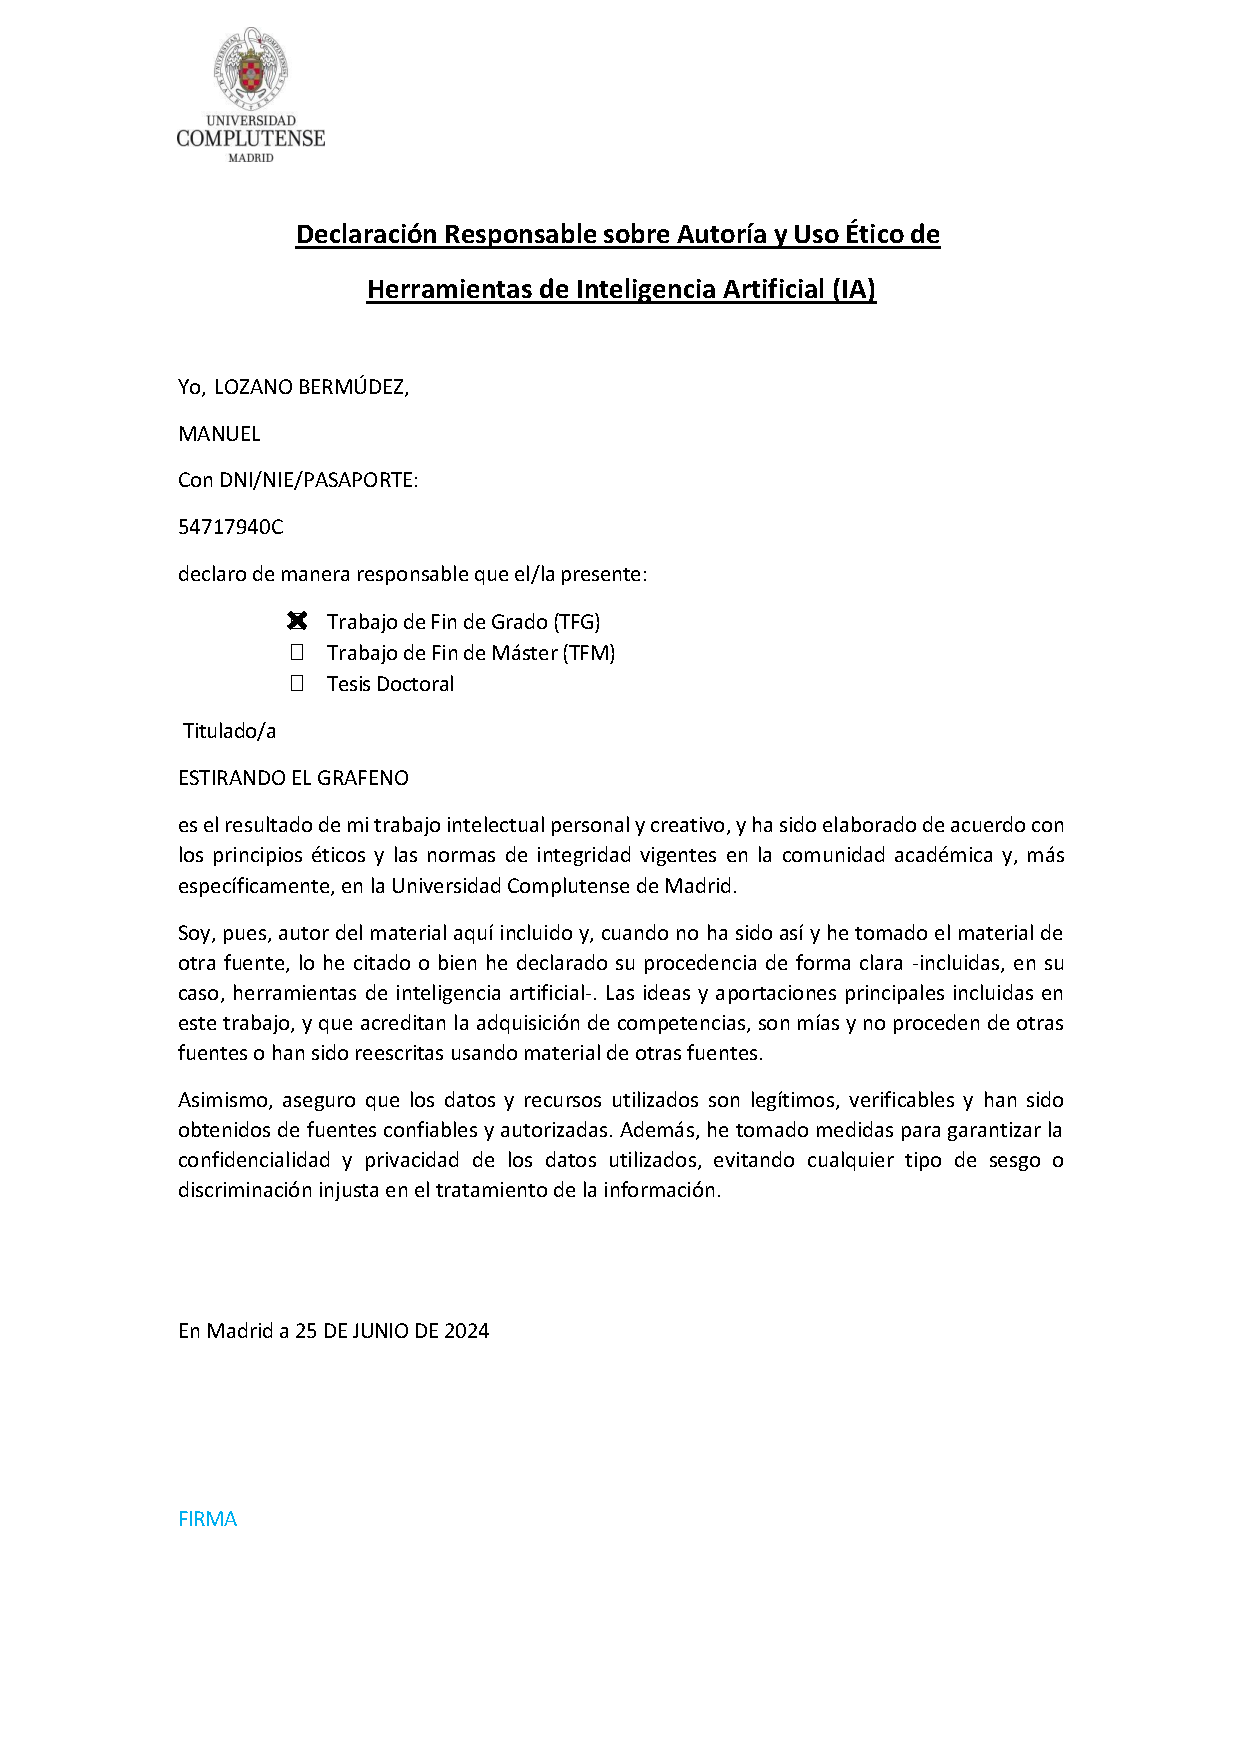
\includepdf[pages=1,pagecommand={},offset=2.5cm -3cm]{ADJUNTOS/declaracion-responsable-sobre-autoria-y-uso-etico-de-ia.pdf}




% \thispagestyle{empty}

% \newpage


%%Inicio:

\pagenumbering{arabic}
\tableofcontents



\newcommand{\arm}{\emph{armchair}}
\newcommand{\zig}{\emph{zigzag}}

\section{Introducción}

El grafeno es uno de los materiales que más ha sido investigado en las últimas décadas y que más atención ha recibido desde su popularización tras su síntesis en 2004 llevada a cabo por primera vez por Geim y Novoselov \cite{science2004}, lo cual les llevaría a recibir el premio Nobel años más tarde. Debido a esta fama, muchos de mi generación, yo incluido, escuchamos su nombre por primera vez en el instituto, seguido de una charla sobre sus muchas y extraordinarias propiedades, simplificadas en gran medida para la comprensión de un adolescente. No obstante, la promesa de innovación tecnológica captó el interés de muchos de nosotros y ha llevado al estudio exhaustivo de este material y la publicación de incontables artículos explorando todas sus posibles aplicaciones; además de dar cabida a multitud de trabajos de final de carrera, como este. \\

Su nombre, acuñado por primera vez en 1986 \cite{BOEHM1986241}, hace referencia a una capa singular de grafito, uno de los muchos materiales alótropos del carbono y que se encuentra abundantemente en la naturaleza y, como caso particular, en las minas de nuestros lápices. Esta monocapa de grafito mantiene una estructura hexagonal o de panal con distancia de aproximadamente $0.142$ nm (o $1.42$ \AA) entre átomos de carbono. Esto se permite gracias a una hibridación de tipo $sp^2$ producida en los orbitales $s$ y $p$ del carbono, que dota a los átomos de una estructura triangular plana, formando enlaces covalentes de tipo $\sigma$ entre ellos. Estos enlaces de tipo $\sigma$ son los que acaban confiriendo al grafeno una gran fortaleza y rigidez, superior a la de cualquier otro material medido, como se vio experimentalmente en 2008 al fijar el módulo de Young del grafeno en $1.0 \pm 0.1 $ TPa \cite{science}. El grafeno también exhibe propiedades electrónicas exóticas, como un gap de semiconductor nulo (densidad de estados nula en el nivel de Fermi). Esta anulación exacta en el nivel de Fermi tiene como consecuencia una relación de dispersión lineal a bajas energías, determinando una región conocida como los \emph{conos de Dirac} (ver Figura \ref{fig:4.0}), en los cuales los electrones, en la banda de conducción, y huecos, en la banda de valencia, se comportan como fermiones relativistas sin masa (o fermiones de Dirac) \cite{castro-neto}. \\
\vspace{-.5cm}
\begin{figure}[!h]
    \centering
    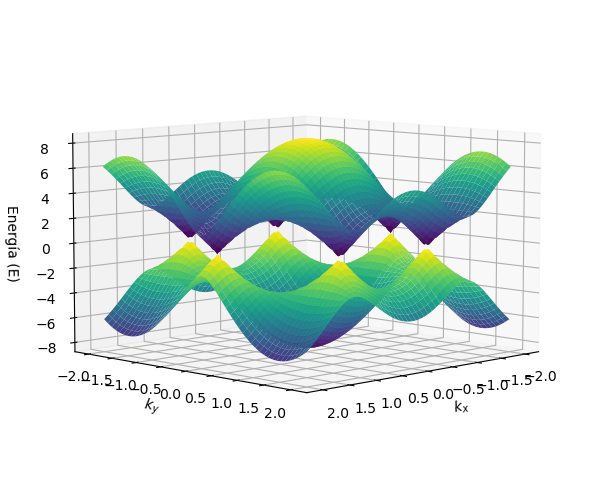
\includegraphics[width = .6\linewidth]{ADJUNTOS/conos-dirac.png}
    % \vspace{-.7cm}
    \caption{Relación de dispersión del grafeno $E(\B{k})$ y conos de Dirac. }
    \label{fig:4.0}
\end{figure}
% No obstante, a pesar de tener una gran cantidad de propiedades, el grafeno presenta un gap nulo de semiconductor, lo que impide poder usarlo en electrónica para la elaboración de circuitos.\\

% Como se ha demostrado en multitud de estudios, una posibilidad para abrir el gap dentro del grafeno puede ser inducir estrés mecánico estirando el grafeno. La ruptura de simetría de la red hexagonal puede modificar la relación de dispersión en los puntos de Dirac, dándonos resultados 

En este trabajo estudiamos las propiedades mecánicas del grafeno, además de explorar la posibilidad de modificar las propiedades electrónicas del grafeno, mediante el estiramiento de la red en la dirección \emph{armchair} (ver Figura \ref{fig:1.1}). Bajo diferentes técnicas de estiramiento y modificando de forma selectiva la red con otros elementos químicos o con defectos estructurales, podremos no sólo cuantificar y comprender mejor las propiedades mecánicas del grafeno sino también la respuesta de romper la simetría hexagonal de la red. Como veremos más adelante, estirar nos permitirá estimar las constantes elásticas del grafeno y conllevará a cambios en la estructura y su estabilidad y en las propiedades electrónicas en determinadas zonas de la red, como se ha comprobado extensamente en experimentos y simulaciones numéricas \cite{PhysRevB.81.241412} \cite{MEMARIAN2015348}\cite{LOPEZPOLIN201742} . \\

\begin{figure}[htbp]
    \centering
    \def\svgwidth{.4\textwidth}
    \input{armchair-zigzag.pdf_tex}
    \caption{Grafeno y las direcciones \emph{armchair} y \emph{zigzag}. }
    \label{fig:1.1}
\end{figure}

Para entender este cambio de las propiedades electrónicas del grafeno, utilizaremos la \textbf{Teoría del Funcional de la Densidad} (\emph{Density Functional Theory}, DFT) a través de simulaciones numéricas. La DFT \cite{sholl} es una teoría usada ampliamente en el ámbito de la física-química e ingeniería para el cálculo de las propiedades electrónicas de un conjunto de átomos como una molécula o parte de una estructura cristalina. En concreto, la DFT se basa en un método variacional que busca la minimización de la energía del estado fundamental del sistema de átomos y electrones por medio de dos teoremas matemáticos fundamentales de la mecánica cuántica aplicada a la física de la materia condensada, conocidos como los \textbf{Teoremas de Hohenberg y Kohn}, que permiten simplificar la ecuación de Schrödinger del sistema de manera significativa. Estos teoremas se estudiarán en las siguientes secciones, así como el código de simulación (FIREBALL) de DFT y sus correspondientes aproximaciones.\\


\section{Objetivos}

El objetivo principal de este trabajo es entender las propiedades mecánicas y cómo cambia la estructura atómica y electrónica del grafeno al realizar estiramientos en la dirección \arm. Para ello, realizamos simulaciones de DFT mediante el código FIREBALL para el cálculo de la estructura para el estado fundamental. Las simulaciones se hacen a temperatura de 0 K, estirando de diferentes maneras hasta alcanzar la ruptura de la red, pudiendo añadir defectos estructurales o dopando la red con átomos de nitrógeno y boro e incorporando también etapas de dinámica molecular a 600 K para simular situaciones de estiramiento más realistas. Finalmente, en diferentes etapas del estiramiento, se calcula la densidad de estados en las regiones cercanas a la de ruptura de la red para realizar contraste y confirmar la apertura del gap de semiconductor. 

\section{Fundamento teórico}

\subsection[Introducción a la DFT]{Introducción a la Teoría del Funcional de la Densidad}

Como se ha comentado anteriormente, el objetivo de la DFT es encontrar el estado de mínima energía de un conjunto de átomos con electrones interactuantes. Para ello, planteamos la ecuación de Schrödinger independiente del tiempo, 

\begin{equation}
    \hat{H} \Phi (\{ \B{r}_i \} , \{ \B{R}_\alpha \}) = E_\text{fund} \Phi (\{ \B{r}_i \} , \{ \B{R}_\alpha \}) \ ; \qquad \B{r}_i , \B{R}_\alpha \equiv \text{posiciones de electrones}  \text{ y núcleos,}
\end{equation}

donde $\Phi$ es la función de onda global del estado fundamental del sistema y $E_\text{fund}$ la energía asociada a ese estado fundamental. El hamiltoniano del sistema tendrá las siguientes contribuciones\footnote{En adelante, usaremos unidades atómicas: $\hbar = e = m_e = 4\pi \varepsilon_0 = 1$.}:

\begin{equation}
    \begin{split}
        \hat{H} = \underbrace{\sum _\alpha \frac{P_\alpha ^2}{2M_\alpha } + \sum _i \frac{p_i^2}{2m_i}}_{(1)} + \underbrace{\frac{1}{2} \frac{1}{4\pi \varepsilon_0} \sum_{i\neq j} \frac{e^2}{|\B{r}_i - \B{r}_j |}}_{(2)} - \underbrace{\frac{1}{4\pi \varepsilon_0} \sum _{i,\alpha } \frac{eZ_\alpha }{|\B{r}_i - \B{R}_\alpha |}}_{(3)} + \underbrace{\frac{1}{2} \frac{1}{4\pi \varepsilon_0} \sum_{\alpha \neq \beta } \frac{Z_\alpha Z_\beta }{|\B{R}_\alpha - \B{R}_\beta |}}_{(4)}
    \end{split}
\end{equation}  

\begin{enumerate}
    \item[(1)] Energías cinéticas de los núcleos atómicos y de los electrones. 
    \item[(2)] Interacción de Coulomb repulsiva entre electrones (de carga $-e$). Tomamos factor $1/2$ para no considerar dos veces la misma interacción.
    \item[(3)] Interacción entre electrones y núcleos atractiva (siendo $Z_\alpha $ el número atómico del núcleo $\alpha$).
    \item[(4)] Interacción entre núcleos repulsiva. 
\end{enumerate}

El problema de Schrödinger de $N$ cuerpos es, en general, intratable tanto analíticamente como computacionalmente. Por lo tanto, es necesario introducir aproximaciones que se justificarán a continuación. 

\subsubsection{Aproximación de Born-Oppenheimer}
Formulada por primera vez por los físicos teóricos Robert J. Oppenheimer y Max Born, se basa en el hecho de que las velocidades de los electrones en la red cristalina de cualquier material es siempre mucho mayor que el movimiento de los iones\footnote{Se hablará indistintamente de núcleos y de iones.}. Esto es debido a que los electrones son muy poco masivos en comparación con los núcleos, por lo que, con respecto a los electrones, la red de iones permanece fija y, respecto a los iones, los electrones responden instantáneamente a su movimiento. Esto permite dar una forma aproximada de la función de onda total del sistema de electrones y núcleos separando ambas contribuciones en un producto de funciones $\Phi(\{ \B{r}_i \} , \{ \B{R}_\alpha \}) = \psi_\text{el}(\{\B{r}_i\}) \psi_\text{nucl}(\{ \B{R}_\alpha \})$. Esto nos permitirá resolver por separado el problema para núcleos y electrones, donde la dificultad ahora residirá en resolver la ecuación de Schrödinger para el estado electrónico, para lo cual los teoremas de Hohenberg-Kohn serán fundamentales.

\subsubsection{Densidad electrónica}
Antes de enunciar los teoremas de Hohenberg-Kohn, debemos introducir la entidad clave que hace que la DFT exista en un primer lugar: la densidad electrónica. En la teoría del funcional de la densidad, intercambiaremos la visión de los electrones como partículas puntuales por la de una densidad electrónica, calculada mecano-cuánticamente según la ecuación \ref{HK}.

\begin{equation} \label{HK}
    \rho(\B{r}) = N \int \left | \psi_\text{el} (\B{r},\B{r}_2,\ldots) \right |^2 \D{\B{r}_2}\ldots \D{\B{r}_N}
\end{equation}

\subsubsection{Teoremas de Hohenberg-Kohn}

Los teoremas de Hohenberg-Kohn (HK) establecen dos propiedades importantes sobre la densidad electrónica que hemos introducido anteriormente. El primero enuncia que \emph{la densidad electrónica determina de forma única el estado fundamental que cumple la ecuación de Schrödinger}. Esto es, en presencia de potenciales externos (por la interacción de los iones y los electrones) del tipo $\upsilon (\B{r}) = -\sum_\alpha Z_\alpha /|\B{r} - \B{R}_\alpha |$, existe un \emph{único} funcional de energía $E = E[\rho]$ para una densidad electrónica dada. Este teorema es un resultado sorprendente y que permite reducir la dimensionalidad del problema electrónico, pasando de tener $N$ electrones a centrarnos en las tres coordenadas espaciales de la densidad electrónica. El segundo teorema HK proporciona una condición a la forma de esta densidad imponiendo que la densidad electrónica que representa al estado fundamental del sistema debe \emph{minimizar el funcional de energía}. Es decir,

\begin{equation}
    E \equiv E[\rho_\text{fund}] \le E[\rho ]
\end{equation}

De este modo, Hohenberg y Kohn proponen un principio variacional para obtener el estado fundamental de la parte electrónica, en el cual $\rho_\text{fund}$ debe hallarse a través de un método de auto consistencia. Con estos dos teoremas, la energía del estado total puede expresarse según la ecuación \ref{tumismo}, separando la contribución que involucra únicamente a los núcleos.

\begin{equation}\label{tumismo}
    E_\text{fund} (\{ \B{R}_\alpha \}) = E[\rho_\text{fund}] + \frac{1}{2} \sum _{\alpha \neq \beta } \frac{Z_\alpha Z_\beta }{|\B{R}_\alpha - \B{R}_\beta |}
\end{equation}
\subsubsection{Ecuaciones de Kohn-Sham}
El siguiente paso es obtener el funcional de energía. Para ello, resulta útil realizar la siguiente aproximación descomponiendo la energía\footnote{La contribución a la energía $E_{\scriptscriptstyle XC}$ se conoce como término de \emph{correlación y canje}. Se comentará más adelante.}:
\begin{align}
    E[\rho] &= \overbrace{\int \upsilon(\B{r}) \rho(\B{r}) \D{\B{r}}}^{\text{el. - núcleo}} + E_{ee}[\rho] + T_S[\rho] + E_{\scriptscriptstyle XC}[\rho] \notag \\
            &= \int \upsilon(\B{r}) \rho(\B{r}) \D{\B{r}} + \frac{1}{2} \iint  \frac{\rho(\B{r}) \rho(\B{r'})}{|\B{r} - \B{r'}|} \D{\B{r},\B{r'}} + T_S[\rho] + E_{\scriptscriptstyle XC}[\rho]
\end{align}
donde $E_{ee}[\rho]$ representa la interacción electrón-electrón -- que escribimos en la forma de densidad de carga -- y $T_S[\rho]$ se define como la energía cinética de los electrones \emph{no interactuantes},
\begin{equation}
    T_S[\rho] = \sum_{n=1}^N \varepsilon_n - \int V(\B{r}) \rho(\B{r}) \D{\B{r}} \ , \qquad \rho(\B{r}) = \sum_{n=1}^N |\psi_n(\B{r})|^2
\end{equation}
donde las funciones de onda monoelectrónicas cumplen la ecuación de Schrödinger, 
\begin{equation} \label{KS}
    \left [ -\frac{1}{2}\laplacian + V(\B{r}) \right ] \psi_n(\B{r}) = \varepsilon_n \psi_n (\B{r})
\end{equation}
Bajo esta premisa, Kohn y Sham demostraron que, al minimizar el funcional de energía respecto de la densidad (tomada como suma de amplitudes de probabilidad de funciones de onda monoelectrónicas), el potencial $V(\B{r})$ de la ecuación \ref{KS} toma necesariamente la siguiente forma.
\begin{align}
    V(\B{r}) &= \upsilon (\B{r}) + \int \frac{\rho(\B{r'})}{|\B{r} - \B{r'}|} \D{\B{r'}} + \fdv{E_{\scriptscriptstyle XC}}{\rho(\B{r})} \equiv \upsilon(\B{r}) + V_H  + V_{\scriptscriptstyle XC} \\
    E_\text{\tiny   KS} [\rho] &= \sum_{n=1}^N \varepsilon_n - E_{ee}[\rho] - \int V_{\scriptscriptstyle XC}(\B{r}) \rho (\B{r}) \D{\B{r}} + E_{\scriptscriptstyle XC} [\rho] \label{func_KS}
\end{align}
De este modo, el problema se reduce a la resolución de $N$ ecuaciones de Schrödinger para las funciones de onda monoelectrónicas, lo que se conoce como aproximación \emph{one electron}, en la que el electrón percibe un potencial promedio producido por el resto de electrones e iones.\footnote{La aproximación \emph{one electron} funciona bien en sistemas en los que la correlación entre electrones es poco importante. En sistemas altamente correlacionados, como sistemas magnéticos, la DFT no produce buenos resultados.}. No obstante, utilizando las ecuaciones de Kohn-Sham vemos que, para determinar la densidad electrónica, tenemos que conocer las funciones de onda monoelectrónicas de primera mano; y que, para determinar las funciones de onda, necesitamos conocer la densidad electrónica, lo cual nos lleva a un argumento circular. Entonces, el procedimiento general para la DFT debe ser el siguiente:

\begin{enumerate}
    \item A partir de una suposición inicial de la densidad electrónica, $\rho_\text{in}$, determinamos el potencial $V_\text{in}(\B{r})$.
    \item A partir del potencial inicial, resolvemos las ecuaciones de Kohn-Sham, obteniendo las funciones monoelectrónicas.
    \item Con las funciones de onda monoelectrónicas, calculamos la densidad electrónica asociada, $\rho_\text{out}$. Con ella, comparamos con la densidad de partida:
    \begin{itemize}
        \item Si las densidades son distintas, repetimos el procedimiento con una densidad que contenga parte de la infomación de la densidad de entrada y de salida. 
        \item Si las densidades son consistentes, podemos calcular la energía y utilizarla para calcular el estado total con contribución electrónica e iónica.
    \end{itemize}
\end{enumerate}
Una vez tenemos la energía, nos queda ocuparnos de la contribución de los núcleos. Las fuerzas electrostáticas inducidas por la densidad electrónica generan un desplazamiento de la red iónica si son muy intensas. Por tanto, se calculan las fuerzas asociadas a esta densidad sobre los núcleos y, si superan un cierto valor umbral, los núcleos se mueven y se reinicia el procedimiento. El bucle de auto consistencia se repite hasta la convergencia de fuerzas y de densidad. 

\subsubsection{Aproximación de pseudo-potencial}
Para reducir la complejidad del método de auto consistencia, incluimos a los electrones de capas más profundas junto con los núcleos atómicos en un nuevo núcleo o \emph{core}. Esta aproximación queda justificada por el hecho de que la mayor parte de las propiedades electrónicas del átomo quedan determinadas por los electrones más externos. La formación del core conlleva un potencial efectivo que, al resolver la ecuación de Kohn-Sham correspondiente, retorna pseudo-orbitales (que dependen de la distancia al core) con un cierto radio de corte\footnote{La elección de este radio de corte no es trivial en absoluto y depende del elemento químico del que se trate.}. A partir del radio de corte, el orbital monoelectrónico recupera el valor original fuera de la aproximación de pseudo-potencial, mientras que, por debajo del radio de corte, decaen de forma suave hasta el origen\footnote{Si, por debajo del radio de corte, las funciones de onda tuviesen ceros ($n>1$), el cálculo de las interacciones se complicaría y no podría hacerse de forma suave.}.

\subsubsection[Aproximación LDA]{Término de canje y correlación y aproximación LDA}
Hasta ahora no hemos hablado de la forma del término de potencial $V_{\scriptscriptstyle XC}$, correspondiente a la energía de correlación y canje de la parte electrónica. En esta contribución se incluyen todos los efectos cuánticos no tenidos en cuenta de la interacción entre electrones, como el efecto de canje producido por el principio de exclusión de Pauli (repulsión efectiva) o las correlaciones entre electrones (que, de forma efectiva, también favorece energéticamente la separación entre electrones). Existen diversas aproximaciones a este término de potencial, pero la más sencilla (y la usada originalmente en el artículo KS) es la de suponer que, en cada punto, la energía por electrón $\varepsilon_{\scriptscriptstyle XC}$ es la misma que la de un gas de electrones de densidad homogénea.

\begin{align}
    \varepsilon_{\scriptscriptstyle XC}(\rho(\B{r})) &= \varepsilon_{\scriptscriptstyle XC}{}^{\text{hom.}}[\rho]\ , \quad \varepsilon_{\scriptscriptstyle XC}{}^{\text{hom.}}[\rho]  \text{ conocido.} \\
    \implies E_{\scriptscriptstyle XC}^\text{\tiny (LDA)}[\rho] &= \int \D{\B{r}} \ \rho(\B{r}) \varepsilon_{\scriptscriptstyle XC}(\rho)\\
    V_{\scriptscriptstyle XC} &= \fdv{E_{\scriptscriptstyle XC}^\text{\tiny (LDA)}[\rho]}{\rho(\B{r})} = \pdv{[\rho(\B{r}) \varepsilon_{\scriptscriptstyle XC}(\rho(\B{r}))]}{\rho(\B{r})}
\end{align}

Esta aproximación se conoce como de densidad local (\emph{Local Density Aproximation}) debido a que se toma la energía de correlación dependiendo únicamente de la posición en el espacio, no de la forma funcional de la densidad. 
% El código FIREBALL utiliza la aproximación LDA calculando las interacciones con las funciones de onda electrónicas de tres centros (como se verá más adelante), pudiendo tabular las integrales y recurrir a ellas para el resto de interacciones mediante interpolación, lo que disminuye el tiempo de cómputo de la simulación significativamente. 
\subsubsection{Teorema de Bloch}
El teorema de Bloch es un resultado central de la física del estado sólido. Bajo la actuación de un potencial periódico (que es el caso de los sólidos cristalinos infinitos), este teorema garantiza que, para un electrón con función de onda $\psi_\B{k} (\B{r}) = \exp(i\B{k}\cdot \B{r}) u_\B{k}(\B{r})$, donde $\B{k}$ es el vector de onda del electrón (puntos de la red recíproca) y $u_\B{k}$ es una función con la misma periodicidad de la red directa; podemos reformular las ecuaciones de Kohn-Sham para pasar de tener un número infinito de átomos y de celdas de la red directa a infinitos puntos $k$ de la red recíproca. Este infinito número de puntos $k$ puede reducirse a un cálculo de un número finito de puntos $k$ especiales que caracterizan la primera zona de Brillouin, simplificando considerablemente el problema \cite{Baldereschi} \cite{Monkhorst}.
\subsection{El código FIREBALL}
Como ya hemos mencionado, FIREBALL es un código de simulación basado en la DFT, que realiza la minimización de la energía del sistema que obedece la ecuación de Schrödinger implementando las aproximaciones vistas anteriormente. Particularmente, se basa en un modelo de electrones fuertemente enlazados (o de \emph{tight-binding}, que se alimenta con parámetros calculados mediante DFT) tomando combinaciones lineales de orbitales atómicos (LCAO, \emph{Linear Combination of Atomic Orbitals}) para construir pseudo-orbitales -- también llamados \emph{fireballs} -- con un radio de corte. El código FIREBALL utiliza la aproximación LDA calculando las interacciones con las funciones de onda electrónicas de tres centros, pudiendo tabular las integrales y recurrir a ellas para el resto de interacciones mediante interpolación, lo que disminuye el tiempo de cómputo de la simulación significativamente. Además, en el método computacional se remplaza el funcional de energía de Kohn-Sham (ecuación \ref{func_KS}) con el funcional de Harris:

\begin{equation}
    E^\text{Harris} [\rho_\text{in}] = \sum_{n=1}^N \varepsilon_n - E_{ee} [\rho_\text{in}] - \int V_{\scriptscriptstyle XC} \rho _\text{in} (\B{r}) \D{\B{r}} + E_{\scriptscriptstyle XC} [\rho_\text{in }] \label{HArris} \ , 
\end{equation}
que únicamente se diferencia del de Kohn-Sham en que utilizamos la densidad electrónica inicial para realizar el cálculo de la energía en vez de la de salida. Esto es lo que nos permite tener a nuestra disposición las interacciones tabuladas para tres centros, como mencionamos anteriormente. Al tomar este funcional, cometemos un error en las energías que de segundo orden con respecto a la diferencia de densiad inicial y de autoconsistencia, $E_\text{H} - E_\text{KS} = \Cl{O}^2(\rho_\text{in} - \rho_\text{AC})$; de modo que, al llegar a la autoconsistencia, la energía del estado fundamental será la misma para el funcional de Harris que para el de Kohn-Sham.  
\subsubsection{Minimización de la energía total}
La minimización de la energía total en el programa FIREBALL puede realizarse a través de dos formas: con el método de los gradientes conjugados (que no usaremos en este caso) y con un método basado en la dinámica molecular. La minimización por dinámica molecular se realiza mediante \emph{dynamical quenching}. En él, se fija la temperatura a 0 K y se deja evolucionar el sistema mientras que la temperatura aumenta al aumentar la energía cinética y la energía potencial disminuye. Cuando la energía potencial sube -- es decir, se produce un \emph{quenching} --, se fija de nuevo la temperatura a 0 K y se continúa con el proceso. Conforme se produzcan procesos de \emph{quenching}, la temperatura incrementará menos hasta que finalmente permanezca a cero, punto en el cual la energía total se habrá minimizado.
% \begin{itemize}
%     \item Gradientes conjugados: La minimización de la energía total del sistema, que en general depende de todas las posiciones atómicas, se realiza variando la energía en las dirección de máximo cambio (gradientes respecto a las posiciones de los átomos). En cada paso, se calcula el gradiente de la energía (equivalente a una fuerza) y se haya el valor de desplazamiento en dirección del gradiente para el cual se minimiza la energía. Este proceso se realiza iterativamente para cada posición atómica, tomando a su vez combinaciones lineales de gradientes de iteraciones anteriores y sucesivas para una convergencia de la energía más rápida. 
 
% \end{itemize}

\section{Metodología y resultados}
Las secciones anteriores han servido para motivar y explicar este trabajo y para tener una base teórica sólida que nos proporcionará las herramientas necesarias para hacer los cálculos. Ahora, introduciremos la metodología utilizada y los resultados de las simulaciones. En primer lugar, determinaremos la distancia entre átomos de carbono de la red de grafeno que utilizará el código FIREBALL para comprobar que es compatible con el valor experimental de 1.42 \AA. Posteriormente, procederemos a simular una celda de tamaño 18x8 de 288 átomos de carbono y estiraremos en pasos sucesivos (desplazamientos de $0.1$ \AA\ de los átomos en cada paso), siempre en la dirección \emph{armchair}, de diferentes maneras (4 casos):
\begin{enumerate}
    \item Estirando en direcciones opuestas de forma rígida por los extremos y permitiendo la relajación (reestructuración de átomos para minimización de la energía) de la red en la región central.
    \item Estirando en direcciones opuestas por la mitad de la red, permitiendo la relajación de la estructura en la región central de la red. 
    \item Estirando de forma rígida los extremos de la red (como en el caso 1) y de forma proporcional a la distancia del centro de la red en la región central.
    \item Estirando de forma idéntica al caso 1 y, al quedar pocos pasos para una ruptura, intercalamos pasos de dinámica molecular (movimiento libre de átomos por acción de la temperatura) y de relajación de la estructura con el estiramiento.
\end{enumerate}
Además de diferentes estiramientos, se introducirán impurezas, como boro o nitrógeno, o defectos, como una vacante y una divacante, en la posición central de la red mientras se estira como en el caso 1. 
\begin{figure}[htbp]
    \centering
    \def\svgwidth{.65\textwidth}
    \input{regiones_graf.pdf_tex}
    \caption{Red de grafeno 18x8 y regiones central y de extremos. La región central tiene un tamaño de 10x8 ($16a$ en la dirección \arm) y los extremos de 4x8 cada uno ($10a$). La celda entera contiene 288 átomos de carbono.}
    \label{fig:enter-label}
\end{figure}

\subsection{Grafeno 1x1 y distancia carbono-carbono}

\begin{figure}[htbp]
    \centering
    \begin{subfigure}{0.41\textwidth}
        \centering
        \def\svgwidth{.8\textwidth}
        \input{base_vdirecta.pdf_tex}
        \caption{Base de grafeno (red directa).}
    \end{subfigure}
    \begin{subfigure}{0.41\textwidth}
        \centering
        \def\svgwidth{.8\textwidth}
        \input{vreciproca.pdf_tex}
        \caption{Primera zona de Brillouin del grafeno.}
    \end{subfigure}
    \caption{Vectores de la red directa $\{ \B{a}_i \}$ y de la red recíproca $\{ \B{b}_i \}$.}
    \label{fig:4.2}
\end{figure}

El objetivo principal, como hemos venido diciendo, es estudiar los efectos del estiramiento en la red de grafeno para determinar sus propiedades mecánicas y elásticas. Antes de ponernos a simular una red de grafeno de gran tamaño, lo ideal es asegurarnos de que nuestro programa toma valores razonables para la distancia de carbono-carbono. La base de grafeno es, como ya hemos visto, hexagonal, con vectores de red $\B{a}_1$ y $\B{a}_2$ que son
\begin{equation}
    \B{a}_1 = a/2 (\sqrt{3}, 1) \quad , \quad \B{a}_2 = a/2 (-\sqrt{3},1) \ .
\end{equation}
La red recíproca tiene como vectores de red a $\B{b}_1$ y $\B{b}_2$, 
\begin{equation}
    \B{b}_1 = \frac{2\pi }{3a} (\sqrt{3}, 1) \quad , \quad \B{b}_2 = \frac{2\pi }{3a} (-\sqrt{3},1) \ .
\end{equation}
En el caso del grafeno, sabemos que $d = 1.42$ \AA; pero FIREBALL, debido a las aproximaciones realizadas, utilizará un valor ligeramente distinto, como veremos a continuación. Comenzaremos realizando unas simulaciones de la base de grafeno de dos átomos de carbono fijos, y variaremos su distancia interatómica en cada simulación para determinar qué parámetro de red minimiza la energía. El resultado es el siguiente.

\begin{figure}[!h]
    \centering
    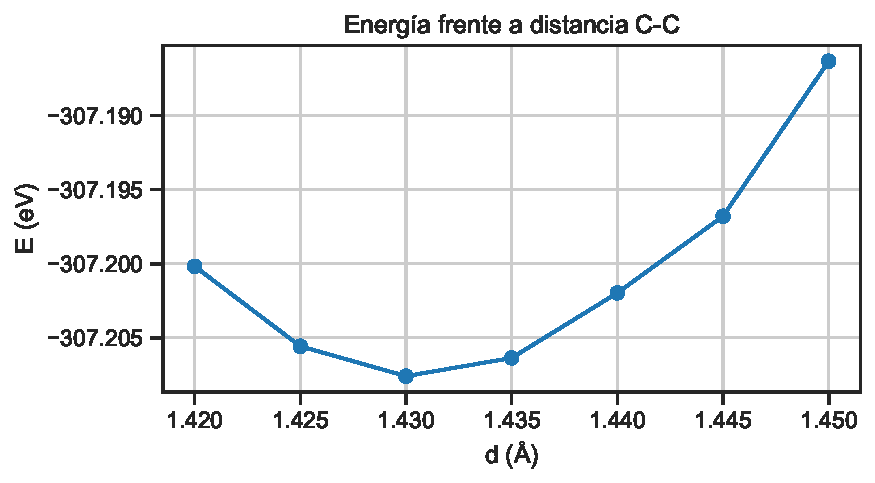
\includegraphics[width = .7\linewidth]{ADJUNTOS/En_param_graf1x1.pdf}
    \caption{Curva de energía de la base de grafeno (1x1) frente a la distancia carbono-carbono. La energía se minimiza para el valor $d = 1.43$ \AA.}
    \label{fig:4.3}
\end{figure}

El valor de la distancia entre carbonos que minimiza la energía -- y que definirá, por lo tanto, a nuestra base de grafeno -- es de $1.43$ \AA\  (error del $0.7\%$). Podemos terminar de verificar que este es el valor apropiado si calculamos la densidad de estados en cualquiera de los átomos de la base. Como puede verse en la Figura \ref{fig:4.4}, distinguimos el ya mencionado cono de Dirac en el nivel de Fermi de la celda 1x1, lo cual confirma que el parámetro tomado por FIREBALL reproduce de forma fiable los resultados teóricos.

\begin{figure}[!h]
    \centering
    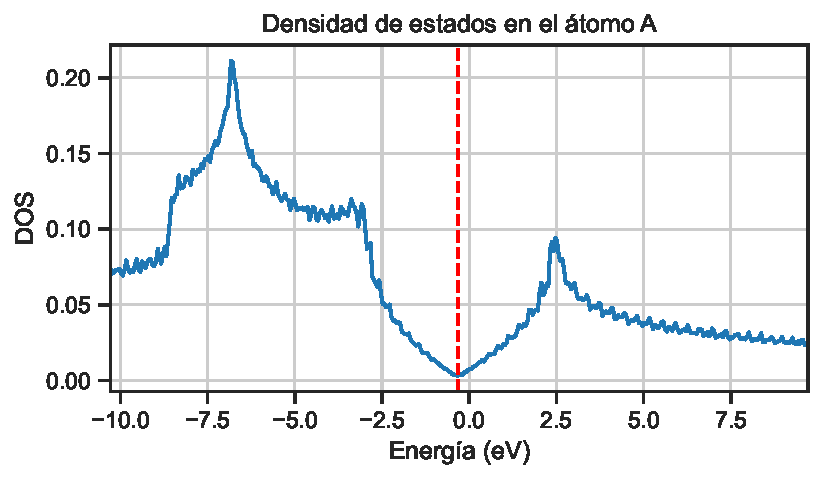
\includegraphics[width = .6\linewidth]{DOS_1x1.pdf}
    \caption{Densidad de estados calculada en el átomo A (ver Figura \ref{fig:4.2}). La línea discontinua representa el nivel de Fermi, $E_F = -0.279$ eV.}
    \label{fig:4.4}
\end{figure}


\subsection{Grafeno 18x8}

Una vez comprobado que la distancia entre carbonos es apropiada para realizar cálculos, podemos comenzar a simular una red de grafeno de mayor tamaño. La red 18x8 tiene como vectores de red:

\begin{equation}
    \B{u}_1 = a (27,0)\quad , \quad \B{u}_2 = a (0,8\sqrt{3}) \quad {\text{\small (dirección \arm orientada en $x$)}}
\end{equation}

En primer lugar, estudiaremos la energía del estado fundamental del grafeno conforme realizamos estiramientos, siguiendo la metodología mencionada anteriormente. 

\subsubsection{Estiramiento rígido} \label{er}
Comenzaremos simulando el estiramiento desplazando de forma rígida los extremos en direcciones opuestas. Cada estiramiento supondrá un desplazamiento en la dirección \arm de $0.1$ \AA \ con respecto a su posición original. De este modo, para cada simulación tomaremos una red desplazada $0.2$ \AA \ con respecto al paso anterior, lo que nos permitirá observar una evolución suave de la energía de la red. Para alcanzar la ruptura, realizamos 26 estiramientos de la red. Dado el gran número de átomos, un número apropiado de puntos $k$ especiales para la relajación (y que no prolongue de forma innecesaria el tiempo de simulación) es de 4 puntos. La energía frente al desplazamiento de la red se puede observar en la Figura \ref{fig:4.5} (a). 
\captionsetup[subfigure]{font={small}, skip=1pt, margin=1cm, singlelinecheck=false}
\begin{figure}[!h]
    \centering
    \begin{subfigure}{0.5\textwidth}
        \caption{}
        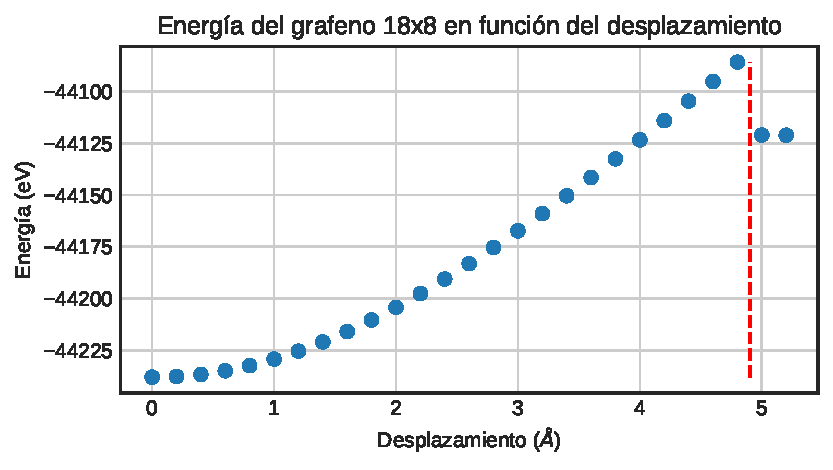
\includegraphics[width = \linewidth]{ADJUNTOS/graf_18x8_en.pdf}
    \end{subfigure}
    \begin{subfigure}{0.487\textwidth}
        \caption{}
        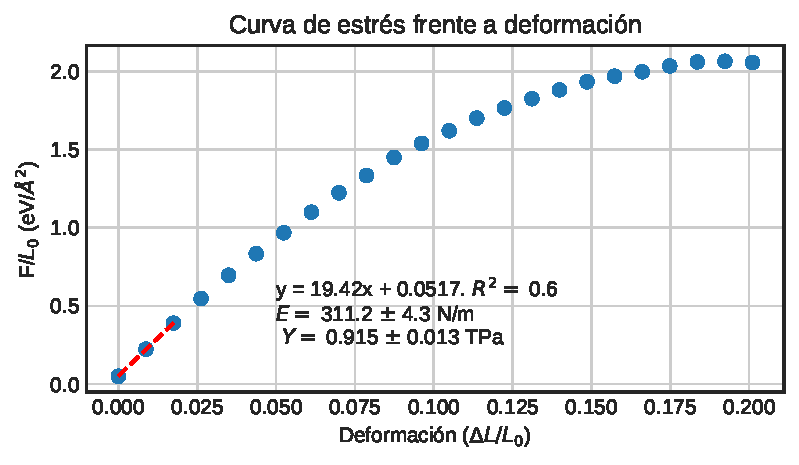
\includegraphics[width = \linewidth]{ADJUNTOS/graf_18x8_young.pdf}
    \end{subfigure}
    \caption{Comportamiento mecánico de la red de grafeno 18x8. a) Energía frente al desplazamiento de la red, b) Estrés frente a deformación de la red. }
    \label{fig:4.5}
\end{figure}

Observamos que, conforme progresan los estiramientos, la energía aumenta hasta un valor máximo, a partir del cual la energía disminuye repentinamente, que coincide con el punto en el cual se alcanza la ruptura de la red. El comportamiento de la energía al estirar el grafeno puede interpretarse dentro de la teoría de elasticidad lineal. Podemos distinguir dos regímenes para la energía: régimen de deformación lineal o simplemente régimen elástico, en el cual las deformaciones aplicadas sobre el grafeno son reversibles y la red retorna a su longitud inicial; y de ruptura, donde se pierde esta reversibilidad y los cambios en la red son permanentes. La fuerza efectiva aplicada sobre la red al modificar las posiciones de los átomos puede tomarse como conservativa y calcularse diferenciando la energía con respecto al desplazamiento. Esta fuerza o estrés ($\sigma$, fuerza partida por la longitud original $L_0$ de la región central\footnote{En materiales 3D, el estrés viene definido como la fuerza por unidad de área transversal a la deformación.}) frente a la deformación $\varepsilon = \Delta L/L_0$ se representa en la Figura \ref{fig:4.5} (b). En la gráfica, observamos que la ruptura se produce para una deformación del 20$\%$ y para un estrés máximo de $32.94$ N/m, que está en acuerdo con resultados previos realizados en DFT\footnote{Cálculos realizados con Quantum Espresso (QE), un código de simulación más preciso pero más lento.} tanto para deformaciones en la dirección \arm como en la \zig \cite{elastic}. El estrés aplicado sobre el material se relaciona con la deformación, en régimen lineal (estrés y deformaciones pequeñas), con el módulo de Young como $\sigma = E \varepsilon$. Por tanto, podemos obtener el módulo de Young (en dos dimensiones) del grafeno como la pendiente de la curva para deformaciones pequeñas, que toma un valor $E = 311$ N/m para nuestras simulaciones. El módulo de Young efectivo puede calcularse finalmente como $Y = E/t$, donde $t$ es el grosor de la red de grafeno\footnote{Tomado como la distancia entre dos láminas de grafito.}. Tomando $t = 3.4$ \AA \ , $Y = 0.915$ TPa. Existen muchos estudios computacionales de las propiedades mecánicas del grafeno que, en función del código de simulación o el modelo físico utilizado para realizar los cálculos (dinámica molecular, modelos continuos, etc.), brindan valores para el módulo de Young distintos. El valor experimental calculado en 2008 \cite{science} se encuentra en $1.0 \pm 0.1 $ TPa, mientras que los métodos computacionales proporcionan valores que se encuentran entre los 0.6 y 1.4 TPa \cite{MEMARIAN2015348}. A pesar de que los ajustes realizados brindan valores del módulo de Young coherentes con los experimentales y son compatibles con los obtenidos mediante otros modelos de simulación, la poca cantidad de datos utilizados no nos permite afirmar con confianza que sean resultados fiables, por lo que un número mayor de puntos (tomando, por ejemplo, más estiramientos con menor desplazamiento) sería más apropiado.\\

Si bien es cierto que, para pequeñas fuerzas aplicadas y pequeñas deformaciones, los materiales presentan un régimen lineal, un análisis más exhaustivo debería tener en cuenta la respuesta mecánica no lineal del grafeno. Este modelo, adoptado por ejemplo en el resultado de Lee \cite{science}, tiene en cuenta órdenes superiores de deformación, teniendo que la tensión mecánica en la dirección \arm es
\begin{equation}
    \sigma = Y \varepsilon + D \varepsilon^2
\end{equation}
donde $Y$ es el módulo de Young y $D$ el módulo elástico de tercer orden. Realizando este ajuste polinómico a todos los datos, obtenemos un valor de $325.9 \pm 1.4$ N/m para el módulo de Young en dos dimensiones y $D = -824.7 \pm 6.5$ N/m (en dos dimensiones), por lo que el módulo efectivo $Y = 0.9584 \pm 0.0040$ TPa, que es una mejoría con respecto a los resultados anteriores, si bien el valor para la constante elástica de tercer orden en dos dimensiones es más pequeña que el valor experimental ($-690 $ N/m), lo cual no es fuera de lo común ya que FIREBALL sobre-estima las interacciones. 

Centrándonos en la estructura resultante después de los estiramientos, en las Figuras \ref{fig:4.19} y \ref{fig:4.6} se puede observar la estructura de grafeno en un paso intermedio de estiramiento y tras la ruptura de la red. 

\begin{figure}[!h]
    \centering
    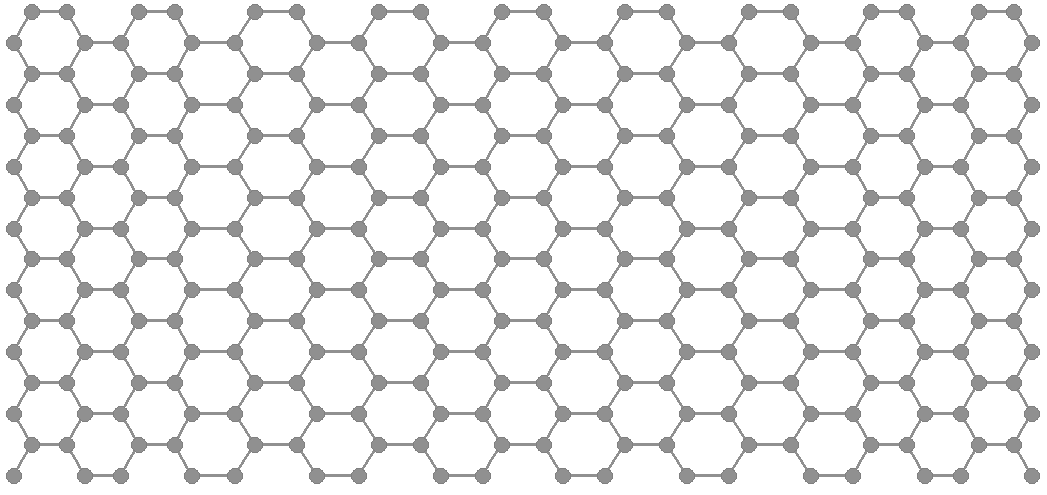
\includegraphics[width = .6\linewidth]{ADJUNTOS/grafeno_a_punto.png}  
    \caption{Estiramiento intermedio. Deformación de la red en la región central.}
    \label{fig:4.19}
\end{figure}
\begin{figure}[!h]
    \centering
    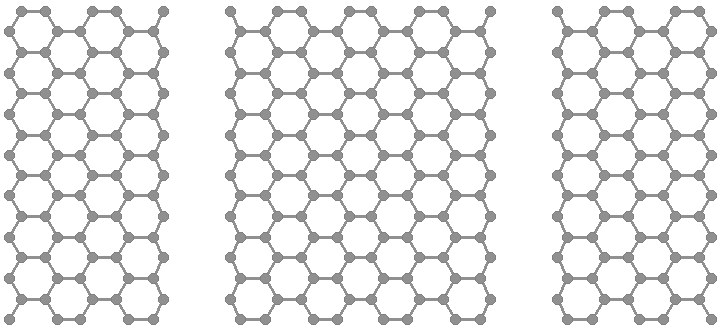
\includegraphics[width = .6\linewidth]{ADJUNTOS/grafeno_roto.png}
    \caption{Red después de la ruptura. Se produce de forma simétrica en ambos extremos.}
    \label{fig:4.6}
\end{figure}

Como era de esperar, la ruptura de la red se produce cerca de la frontera entre el extremo y la región central, que es donde hay una ruptura de la simetría de la red hexagonal. Se produce además de forma simultánea en ambos extremos al producirse el estiramiento de forma simétrica.\\


Por último, podemos comparar la densidad de estados de los átomos de la región central para observar un cambio en las propiedades electrónicas del grafeno (calculando con 64 puntos $k$ especiales). En concreto, consideramos dos estiramientos, uno intermedio (con distancia entre átomos de carbono del centro de la red $d = 1.65$ \AA) y otro pocos pasos antes de la ruptura ($d = 1.75$ \AA), y comparamos con la densidad de estados teórica del grafeno sin estirar . Como puede comprobarse en la Figura \ref{fig:4.16}, el estiramiento tiene el efecto de modificar la densidad de estados, teniendo un valor no nulo en el nivel de Fermi y formándose un gap, si bien las curvas de densidad de estados tienen bastante distorsión. Esto es debido a que se ha utilizado un número de puntos $\B{k}$ de la primera zona de Brillouin insuficientes, lo cual genera ondulaciones en las curvas de DOS. Para poder determinar con precisión esta apertura de gap, sería necesario recalcular las densidades de estados con mayor número de puntos (esto es, dedicando un mayor tiempo de cómputo).  


\begin{figure}[!h]
    \centering
    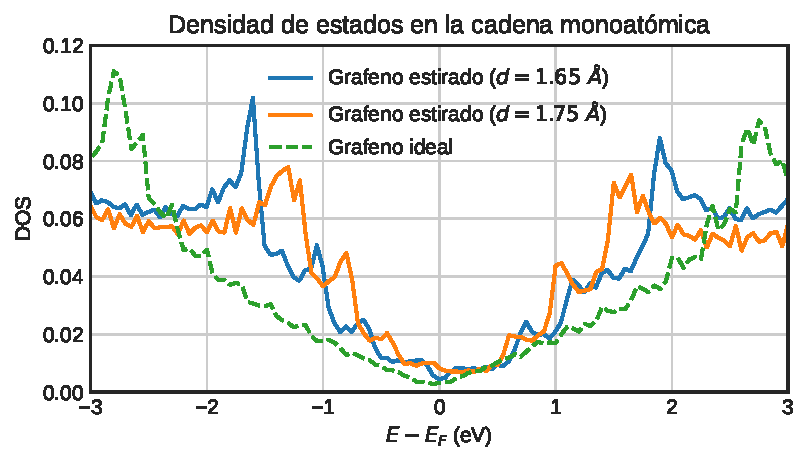
\includegraphics[width = .7\linewidth]{ADJUNTOS/DOS_graf18x8_int_av_141.pdf}
    \caption{Efecto del estiramiento en la densidad de estados del grafeno. }
    \label{fig:4.16}
\end{figure}

\subsubsection{Comparación de métodos de estiramiento}
En la siguiente sección comentamos la estabilidad que tienen diferentes métodos de estiramiento en comparación con el estiramiento por los extremos de forma rígida. En concreto, analizamos dos formas de estirar alternativas: desplazando la red por mitades en direcciones opuestas y relajando la red, manteniendo fijos los átomos de los extremos; y estirando por los extremos de forma rígida además de desplazar los átomos de la región central en direcciones contrarias un pequeño porcentaje (que es proporcional a la distancia a los extremos), dejando que la estructura relaje fijando los extremos como anteriormente. El primer método (estiramiento por el centro) nos permite distinguir si resulta más viable energéticamente romper la simetría en otra parte de la red que en los extremos; y el segundo nos permite simular un caso de estiramiento progresivo ligeramente más realista que el caso de un desplazamiento repentino únicamente de los extremos. Para este último, los átomos del centro de la red permanecerán inmóviles mientras que el resto se desplazarán en incrementos del $10\%$ del desplazamiento original (que es $0.1$ \AA. Es decir, $0.01$ \AA \ para la primera columna de átomos, $0.02$ \AA \ la segunda, etc.). En la Figura \ref{fig:4.7} se ven representadas las energías (respecto a su energía inicial) para los tres métodos mencionados para 20 estiramientos (desplazamiento total de $4$ \AA).  \\

\begin{figure}[!h]
    \centering
    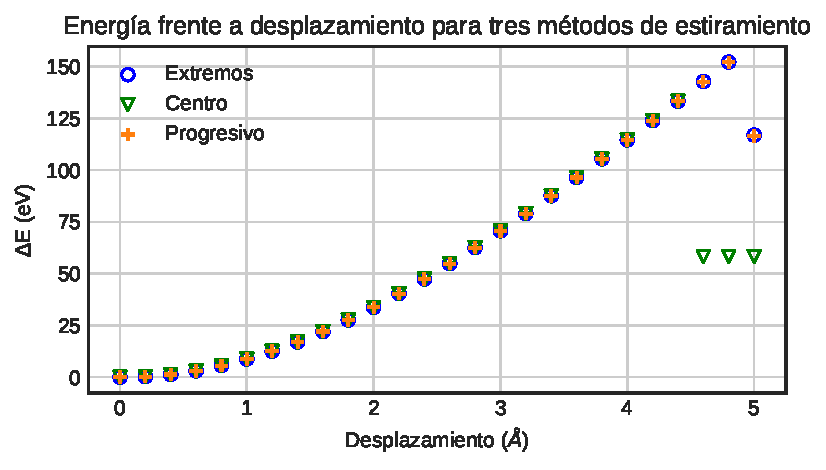
\includegraphics[width = .7\linewidth]{ADJUNTOS/graf_18x8_comp_en.pdf}
    \caption{Comparación de métodos de estiramiento de la red de grafeno 18x8.}
    \label{fig:4.7}
\end{figure}

\begin{figure}[!h]
    \centering
    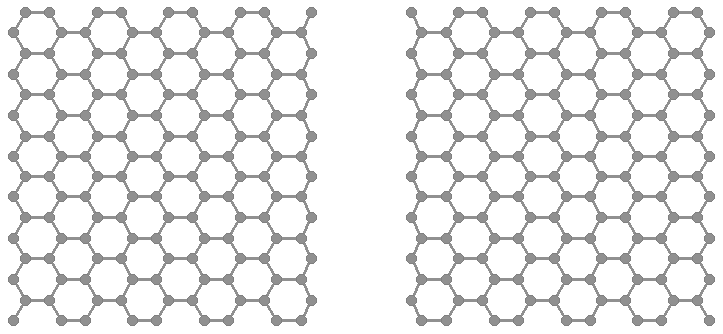
\includegraphics[width = .6\linewidth]{ADJUNTOS/roto_centro.png}
    \caption{Estructura final tras estirar por el centro de la red.}
    \label{fig:4.8}
\end{figure}

Como se puede comprobar, la energía en las primeras etapas del estiramiento es la misma independientemente de qué método de estiramiento escojamos. Este resultado es lo esperable ya que, al no modificarse en gran medida la forma de la estructura, la relajación de la red después de estirar acaba por retornar el mismo estado fundamental en los tres casos, distribuyendo la deformación entre todos los enlaces. No obstante, al estirar por el centro la red acaba por romperse antes, acabando en un estado de mucha menor energía que en los dos casos anteriores. Si observamos la estructura final (Figura \ref{fig:4.8}) estirando por el centro, vemos que la ruptura se produce en el centro de la red. En el caso del estiramiento por los extremos, acabamos rompiendo dos cadenas de enlaces, dando lugar a tres subsistemas; mientras que en este estiramiento solo rompemos una cadena de enlaces. Es lógico por tanto concluir que el método de estiramiento de la red más estable es por el centro.

\subsubsection{Estiramiento con dinámica molecular}

El último método de estiramiento que consideramos en este trabajo combina el estiramiento de la red por los extremos con pasos de dinámica molecular para desorganizar la red antes de cada estiramiento. Las simulaciones realizadas anteriormente, si bien son coherentes con lo esperado a temperatura nula, no reflejan de forma adecuada la situación real de deformación de una lámina de grafeno, en la cual la temperatura, ya no nula, juega un papel central en la reorganización de la red para la minimización de la energía al introducir asimetrías puntuales, que pueden llevarnos a situaciones de ruptura distintas. Para simular este estiramiento realista, realizamos estiramientos centrales vistos anteriormente hasta que la red se encuentre cerca de la ruptura. A partir de este punto, introducimos una temperatura (600 K) y dejamos evolucionar el sistema de forma libre durante una serie de pasos (500). Posteriormente, relajamos la estructura y continuamos estirando y relajando. Repetimos este proceso de dinámica molecular-relajación-estiramiento-relajación hasta alcanzar la ruptura de la red. Los resultados de este procedimiento se ven en las Figuras \ref{fig:4.9} y \ref{fig:4.10}. \\

Lo primero que observamos al analizar las energías es que la ``ruptura'' se produce antes estirando y desorganizando la red por dinámica molecular que si solamente estiramos por los extremos. La energía durante los últimos pasos son iguales en ambos casos, pero las energías después de la ruptura en ambos casos indican que el estiramiento con pasos de dinámica nos lleva a estructuras más estables que en caso contrario. \\

\begin{figure}[!h]
    \centering
    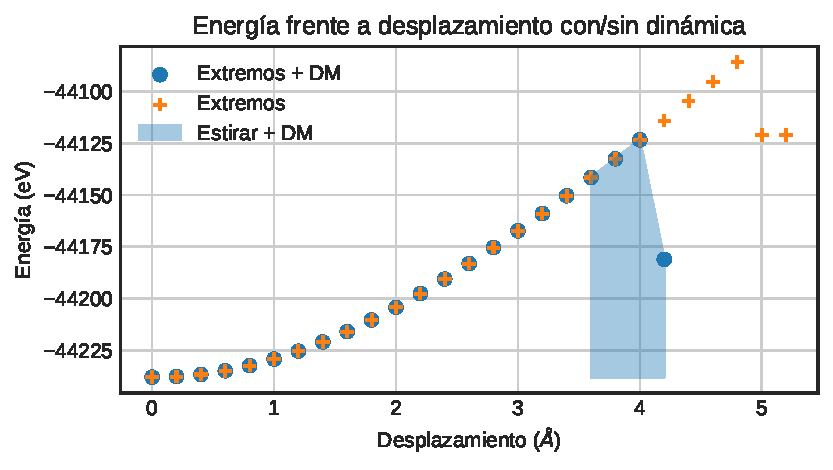
\includegraphics[width = .7\linewidth]{ADJUNTOS/graf_18x8_v5_en.pdf}
    \caption{Comparación de energía estirando con y sin dinámica molecular (MD).}
    \label{fig:4.9}
\end{figure}

\begin{figure}[!h]
    \centering
    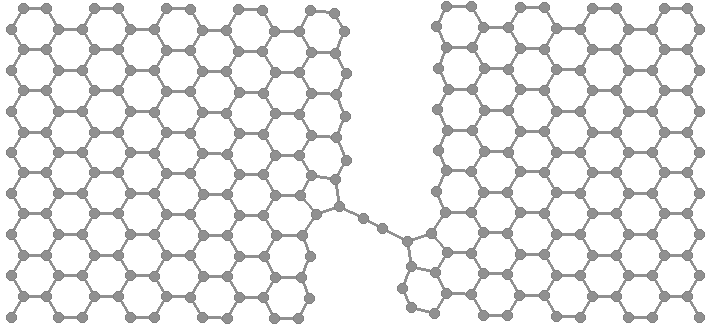
\includegraphics[width = .6\linewidth]{ADJUNTOS/cadena-mono.png}
    \caption{Red de grafeno tras estirar con dinámica molecular y formación de una cadena monoatómica.}
    \label{fig:4.10}
\end{figure}

Lo más interesante de este método de estiramiento es la estructura final resultante. En este caso, podemos ver que la ruptura de la red está incompleta y que se ha formado una cadena monoatómica entre ambas secciones. Es un resultado completamente distinto al de los otros tres métodos de estiramiento pero que es más coherente con una situación realista de estiramiento de grafeno, en la que el efecto de la temperatura reordena los átomos permitiendo que alcancen nuevas configuraciones de mínima energía, en este caso una cadena de átomos. Dado que la dinámica molecular es un proceso inherentemente aleatorio, al volver a simular este procedimiento es posible que obtengamos una estructura distinta de la observada. Esto puede dar paso a seguir estudiando la formación de estas estructuras, repitiendo las simulaciones para mismas condiciones y poder así hacer estadística o en diferentes condiciones de estiramiento y de temperatura para explorar nuevas posibles estructuras. \\

Podemos fijarnos en la densidad de estados en los átomos de la cadena monoatómica, como se ve en la Figura \ref{fig:4.17}. Nos encontramos con un gran pico de densidad en la región cercana al nivel de Fermi. La presencia de este pico tiene consecuencias en las propiedades electrónicas de la cadena de átomos, ya que, al haber electrones ocupando estados cercanos al nivel de Fermi, se puede dar la posibilidad de conducción entre ambas regiones conectadas por la cadena monoatómica; además de hacer la cadena reactiva, por lo que otra futura línea de trabajo puede ser estudiar la interacción de esta estructura con otros átomos o moléculas. \\

\begin{figure}[!h]
    \centering
    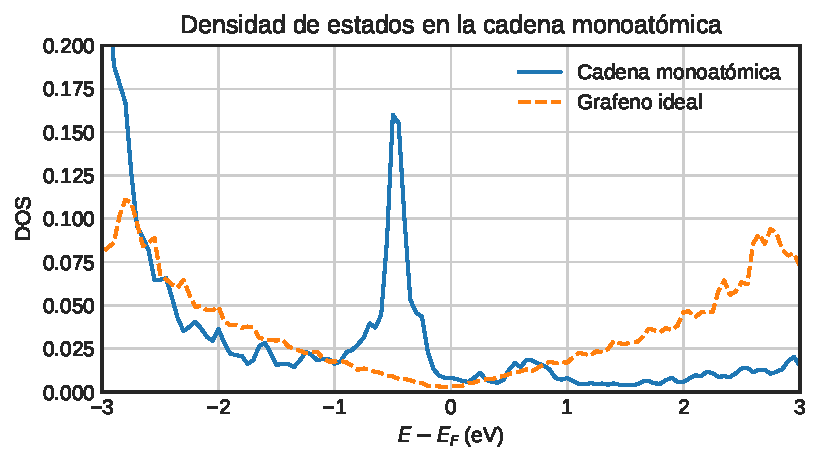
\includegraphics[width = .7\linewidth]{ADJUNTOS/DOS_graf18x8_cadena.pdf}
    \caption{Densidad de estados en la cadena monoatómica.}
    \label{fig:4.17}
\end{figure}

\subsection{Grafeno 18x8 con defectos}
En esta sección, analizaremos el efecto de introducir dos defectos en la red en sus propiedades mecánicas. En este caso, introducimos una vacante y divacante (uno y dos huecos) en la red y estiramos por los extremos hasta alcanzar la ruptura. Los resultados se ilustran en las Figuras \ref{fig:4.11}, \ref{fig:4.14} y \ref{fig:4.15}. \\

\begin{figure}[!h]
     \centering
     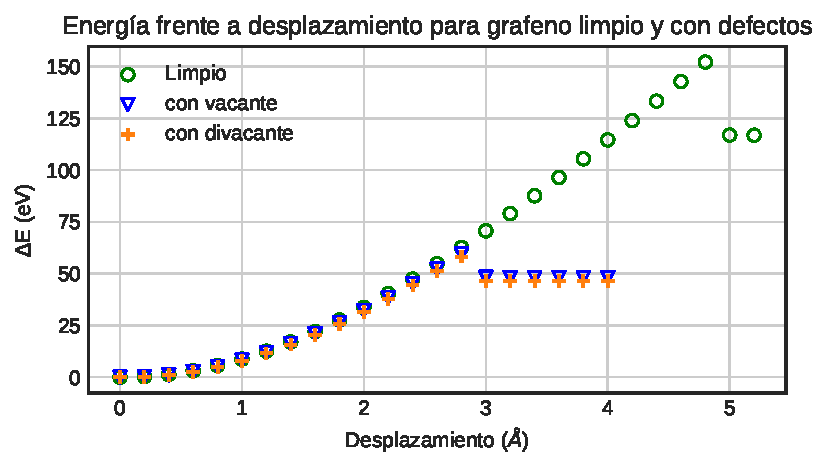
\includegraphics[width = 0.7\linewidth]{ADJUNTOS/graf_18x8_v1-vac-divac_en.pdf}
     \caption{Comparación de energías del grafeno ``limpio'' y con vacante y divacante.}
     \label{fig:4.11}
 \end{figure}

\begin{figure}[!h]
    \centering
    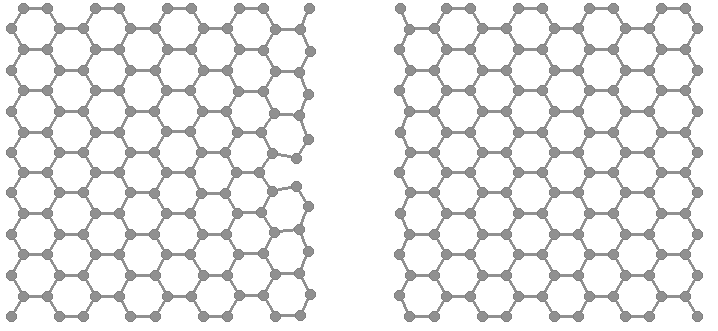
\includegraphics[width = .6\linewidth]{ADJUNTOS/roto_vacante.png}
    \caption{Estructura final de la red de grafeno con una vacante}
    \label{fig:4.14}
\end{figure}

\begin{figure}[!h]
    \centering
    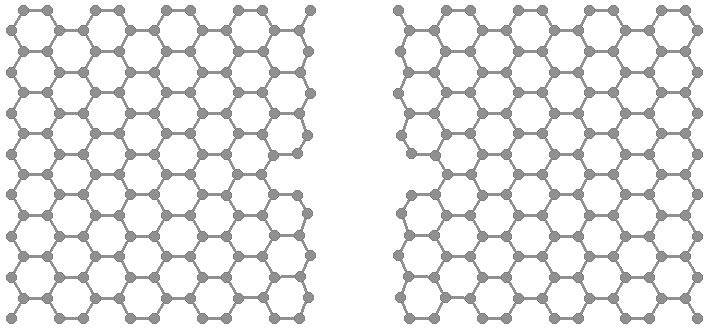
\includegraphics[width = .6\linewidth]{ADJUNTOS/roto_divacante.png}
    \caption{Estructura final de la red de grafeno con dos vacantes. }
    \label{fig:4.15}
\end{figure}

La progresión de la energía es muy similar para la red de grafeno limpia como para las redes con defectos. La ruptura, sin embargo, se produce mucho antes en el caso de la red con defectos que en la red normal, alcanzándose en ambos casos a $3.0$ \AA \ de elongación con respecto a la longitud inicial. De hecho, esta ruptura se produce incluso antes que en el caso del boro ($4.2$ \AA) y del nitrógeno ($3.8$ \AA), como veremos más adelante. Esto es debido a que, con dopantes, existen enlaces -- si bien son débiles -- con el carbono que desaparecen al introducir una vacante (3 en el caso de la vacante, 6 con la divacante). Esto genera una cierta inestabilidad estructural que favorece la ruptura de la red. Calculando el módulo de Young efectivo (en el caso de la divacante), obtenemos un valor de $Y = 0.892 \pm 0.016 $ TPa, ligeramente inferior al de la red ideal, mientras que con el ajuste cuadrático obtenemos un módulo efectivo de $0.974 \pm 0.020$ TPa. La disparidad entre ambos valores para la divacante puede deberse a la falta de puntos a mayores deformaciones debido a la temprana ruptura de la red, por lo que sería necesario un cálculo con menor desplazamiento en cada estiramiento.


\subsection{Grafeno 18x8 dopado}

Finalmente, estudiaremos el efecto de dopar la red de grafeno con un átomo de boro o de nitrógeno mientras estiramos por los extremos. Tanto el boro, con tres electrones en su capa de valencia, como el nitrógeno, con cinco electrones, cambiarán la distribución de las cargas de la región próxima al dopante, de manera que la simetría entre los enlaces con los carbonos se romperá y generarán una inestabilidad que tendrá consecuencias en el estiramiento de la red. En ambos casos, el dopante sustituirá al átomo de la posición central de la red, y se procederá a estirar el retículo de la misma forma que se planteó en la sección \ref{er}. Los resultados tanto para el boro como para el nitrógeno se representan en la Figura \ref{fig:4.11}.
 \begin{figure}[!h]
     \centering
     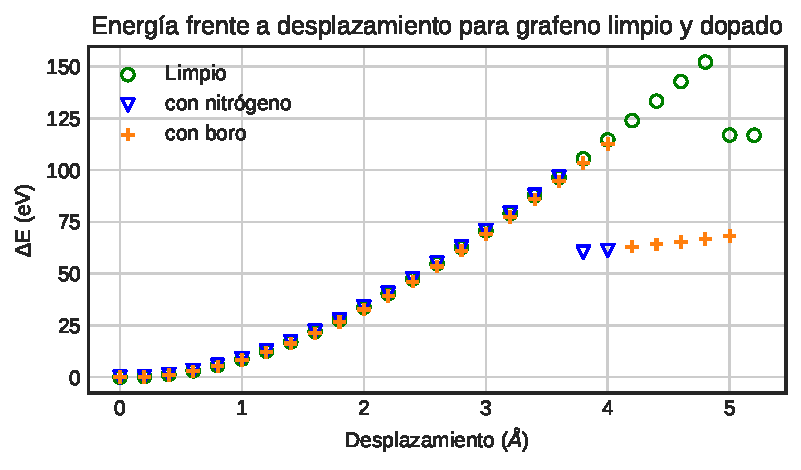
\includegraphics[width = 0.7\linewidth]{ADJUNTOS/graf_18x8_v1-nit-bor_en.pdf}
     \caption{Comparación de energías del grafeno ``limpio'' y dopado con boro y nitrógeno.}
     \label{fig:4.11}
 \end{figure}
En la gráfica vemos que la progresión de la energía para las tres redes de grafeno son muy parecidas hasta el estiramiento $\#$18, a partir del cual el grafeno con nitrógeno se rompe; seguido del boro dos pasos después. Vemos entonces que dopar la red de grafeno, si bien es estable, acaba rompiéndose antes debido a esta ruptura de simetría. Un cálculo de estrés en la red por deformación como en la sección \ref{er} nos permite calcular el módulo de Young efectivo de la red con boro y con nitrógeno, dando como resultado $0.921 \pm 0.019$ TPa para el caso del boro y de $0.917 \pm 0.015$ TPa. Un ajuste cuadrático a la curva entera nos proporciona los siguientes valores: para el nitrógeno, $0.9623 \pm 0.0076$ TPa y para el boro, $0.9505 \pm 0.0094$ TPa, que son ambos muy cercanos al valor de la red de grafeno limpio.\\

Fijándonos en las estructuras resultantes (Figuras \ref{fig:4.12} y \ref{fig:4.13}), vemos que en ambos casos la estructura se rompe por el centro de la red, en la región del dopante. Este resultado, como hemos comentado antes, se debe a la ruptura de la simetría de la red en el enlace boro-carbono o nitrógeno-carbono, haciendo que sea más beneficioso energéticamente romper la red por el centro en vez de los extremos, como en el caso del grafeno limpio. Por último, vemos también que, en ambos casos, se forman cadenas de átomos de carbono en las partes más alejadas del dopante en la zona de la ruptura. Como en el caso de dinámica molecular con el grafeno limpio, puede ser interesante seguir estudiando la formación de estas cadenas en diferentes condiciones de estiramiento e introduciendo temperatura, además de sus propiedades electrónicas. 

\begin{figure}[!h]
    \centering
    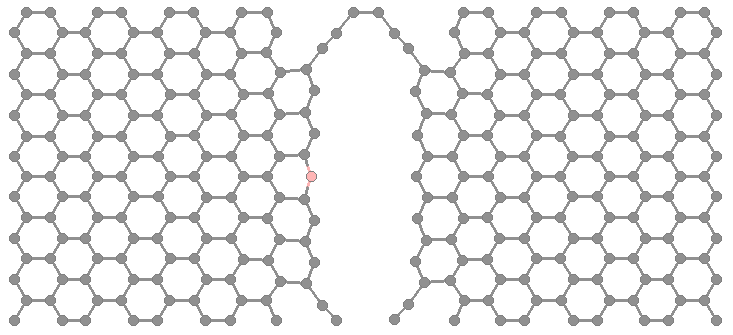
\includegraphics[width = .6\linewidth]{ADJUNTOS/roto_boro.png}
    \caption{Estructura final de grafeno con boro.}
    \label{fig:4.12}
\end{figure}

\begin{figure}[!h]
    \centering
    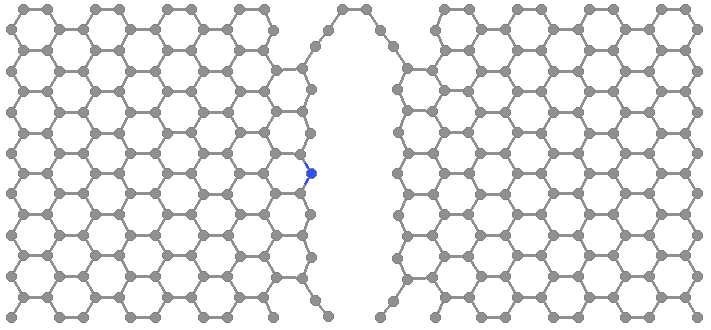
\includegraphics[width = .6\linewidth]{ADJUNTOS/roto_nitro.png}
    \caption{Estructura final de grafeno con nitrógeno.}
    \label{fig:4.13}
\end{figure}



% \subsection{Grafeno 18x8 con defectos}
% De la misma manera que con los dopantes, introduciremos dos defectos en la red para estudiar sus propiedades mecánicas. En este caso, introducimos una vacante y divacante (uno y dos huecos) en la red y estiramos por los extremos hasta alcanzar la ruptura. Los resultados se ilustran en las Figuras \ref{fig:4.11}, \ref{fig:4.14} y \ref{fig:4.15}. \\

% \begin{figure}[!h]
%      \centering
%      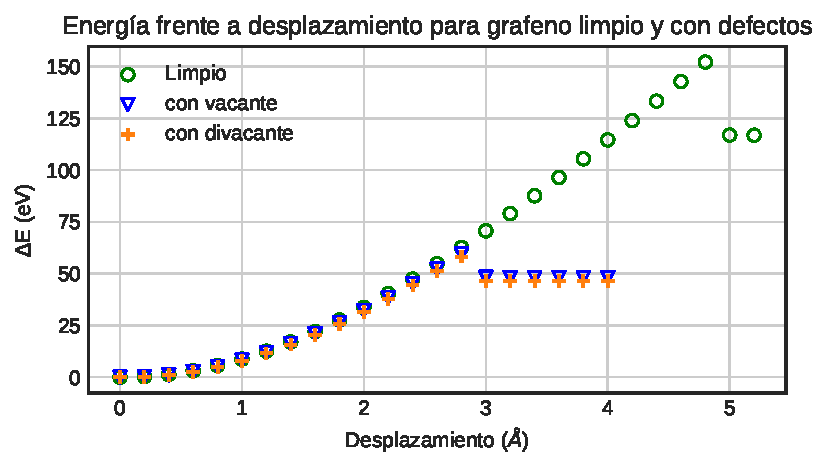
\includegraphics[width = 0.7\linewidth]{ADJUNTOS/graf_18x8_v1-vac-divac_en.pdf}
%      \caption{Comparación de energías del grafeno ``limpio'' y con vacante y divacante.}
%      \label{fig:4.11}
%  \end{figure}

% \begin{figure}[!h]
%     \centering
%     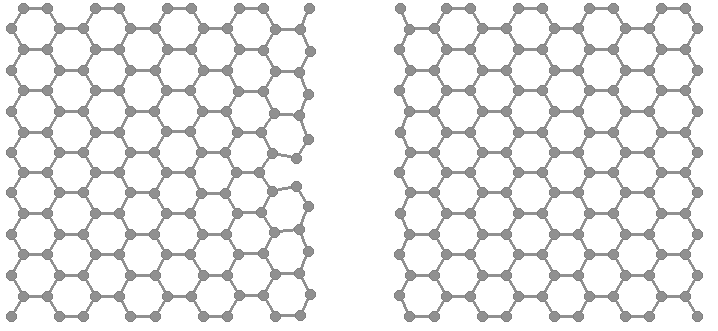
\includegraphics[width = .6\linewidth]{ADJUNTOS/roto_vacante.png}
%     \caption{Estructura final de la red de grafeno con una vacante}
%     \label{fig:4.14}
% \end{figure}

% \begin{figure}[!h]
%     \centering
%     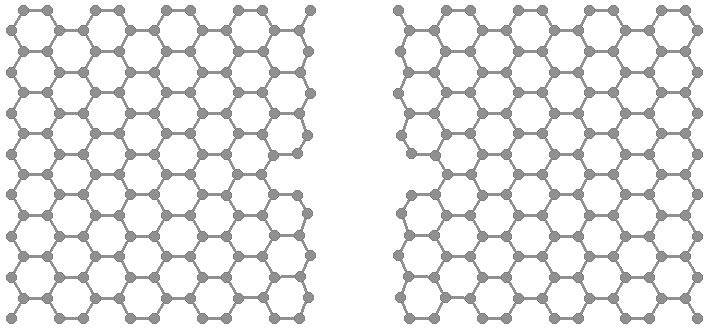
\includegraphics[width = .6\linewidth]{ADJUNTOS/roto_divacante.png}
%     \caption{Estructura final de la red de grafeno con dos vacantes. }
%     \label{fig:4.15}
% \end{figure}

% Como en casos anteriores con dopantes, la progresión de la energía es idéntica para la red de grafeno limpia como para las redes con defectos. La ruptura, sin embargo, se produce mucho antes en el caso de la red con defectos que en la red normal, alcanzándose en ambos casos a $3.0$ \AA \ de elongación con respecto a la longitud inicial. De hecho, esta ruptura se produce incluso antes que en el caso del boro ($4.2$ \AA) y del nitrógeno ($3.8$ \AA). Esto es debido a que, con dopantes, existen enlaces -- sin bien son débiles -- con el carbono que desaparecen al introducir una vacante (3 en el caso de la vacante, 6 con la divacante). Esto genera una gran inestabilidad estructural que favorece la ruptura de la red. Calculando el módulo de Young efectivo (en el caso de la divacante), obtenemos un valor de $Y = 0.892 \pm 0.016 $ TPa, ligeramente inferior al de la red ideal, que es una manifestación de esa inestabilidad estructural.    


\newpage
\section{Conclusiones}

A lo largo de este trabajo, hemos revisado los fundamentos físicos de la Teoría del Funcional de la Densidad, además de las aproximaciones principales realizadas, y hemos puesto en práctica el modelo estudiando el efecto del estiramiento de una red de grafeno en sus propiedades mecánicas y electrónicas. Utilizando el código FIREBALL, basado en la teoría DFT y la dinámica molecular, y un modelo sencillo de desplazamiento de la red atómica, hemos reproducido el efecto del estiramiento de la red y hemos deducido diversas propiedades mecánicas de este material, como el módulo de Young, y comparado con éxito con resultados experimentales y de otras simulaciones realizadas con otro programa de cálculo utilizado dentro del marco teórico de la DFT, Quantum Espresso, que, si bien es más preciso, requiere muchos más recursos para realizar el cálculo (típicamente realizado en supercomputadores), a diferencia del programa FIREBALL, que puede realizar los cálculos desde un ordenador de sobremesa. Hemos estudiado diferentes técnicas de estiramiento y su estabilidad, además de analizar el efecto de los dopantes (boro y nitrógeno) y los defectos estructurales (vacante y divacante) e interpretando las diferentes estructuras resultantes, como cadenas de átomos de carbono. A su vez, hemos calculado la densidad de estados en diferentes etapas de los estiramientos, apreciando un cambio importante respecto a la densidad de estados del grafeno ideal alrededor del nivel de Fermi en donde parece formarse un gap, como ha sido posible confirmar en experimentos. Por último, también hemos propuesto reactividad en las cadenas monoatómicas al analizar la densidad de estados. \\


% En experimentos ha sido posible confirmar una apertura de gap, por lo que sería necesario mejorar el cálculo de la densidad de estados para confirmar este resultado con nuestro modelo de estiramiento
% Cabe comentar los resultados del módulo de Young obtenidos. Si bien los ajustes realizados brindan valores del módulo de Young coherentes con los experimentales y son compatibles con los obtenidos mediante otros modelos de simulación, la poca cantidad de datos utilizados junto con la pobreza del ajuste ($R^2 = 0.6$) no nos permiten afirmar con confianza que sean resultados fiables. Si bien es cierto que, para pequeñas fuerzas aplicadas y pequeñas deformaciones, los materiales presentan un régimen lineal, un análisis más exhaustivo debería tener en cuenta la respuesta mecánica no lineal del grafeno. Este modelo, adoptado por ejemplo en el resultado de Lee \cite{science}, tiene en cuenta órdenes superiores de deformación, teniendo que la tensión mecánica en la dirección \arm es
% \begin{equation}
%     \sigma = Y \varepsilon + D \varepsilon^2
% \end{equation}
% donde $Y$ es el módulo de Young y $D$ el módulo elástico de tercer orden. Esta implementación de modelo de elasticidad sería interesante para realizar trabajos futuros, pero por cuestiones de tiempo y de dificultad no ha sido posible introducirlo en este trabajo. 

En general, para futuros trabajos a partir de este proyecto se abre un gran abanico de posibilidades, como determinar en qué condiciones específicas se forman las cadenas monoatómicas al romper mediante dinámica molecular, así como estudiar la capacidad de captación de átomos o de moléculas por estas cadenas monoatómicas. Como conclusión final a esta memoria, este trabajo es la convergencia de muchas líneas de trabajo, de ideas propuestas y, sobre todo, de muchos errores e intentos fallidos; que han sido las lecciones de las cuales más he aprendido en el desarrollo de este proyecto. Más allá de la física aprendida o de los resultados obtenidos, me ha proporcionado una exposición de primera mano a la labores de investigación básicas que se realizan en todos los campos de la física y, en general, de la ciencia. Por último, representa tanto un punto final a mis estudios de grado como un nuevo punto de partida para seguir formándome en el área de la física computacional. 

\newpage

\addcontentsline{toc}{section}{Referencias}

\printbibliography

\end{document}

